%!TEX root = ../Thesis.tex
\chapter{Analytical Mechanics} \label{ch:analytical-mechanics}
\epigraph{``\itshape{If Nature has defined the mechanics problem of the thrown ball in so elegant a fashion, might She have defined other problems similarly. So it seems now. Indeed, at the present time it appears that we can describe all the fundamental forces in terms of a Lagrangian. The search for Nature's One Equation, which rules all of the universe, has been largely a search for an adequate Lagrangian.}"}{--- \textup{Robert Adair}, The Great Design: Particles, Fields, and Creation}


%%%%%%%%%%%%%%%%%%%%%%%%%%%%%%%%%%%%%%%%%%%%%%%%%%%%%%%%%%%%%%%%%%%%%%%%%%%%%%
\section{Newtonian Mechanics}
Since the early beginnings of classical mechanics, there have existed fundamentally two different approaches to the study of motion: vectorial (``classical'') and variational (``analytical'') treatment of mechanics. The first, a differential approach, the second, an integral approach.

The vectorial treatment was pioneered by Isaac Newton and is based on two fundamental vectors: momentum and force. Analysis of the forces acting on a body yield second-order differential equations of motion by Newton's 2nd Law, equation \eqref{eq:newton2}. These differential equations can be solved to yield position and velocity at every point in time:
\begin{align}
\label{eq:newton2}
\textbf{Newton's 2nd Law} \qquad \sum{\vec{F}} = \dfrac{d \vec{p}}{dt}.
\end{align}


%%%%%%%%%%%%%%%%%%%%%%%%%%%%%%%%%%%%%%%%%%%%%%%%%%%%%%%%%%%%%%%%%%%%%%%%%%%%%%
\section{Lagrangian Mechanics}
The first seeds of the variational approach was sown by G.W. Leibniz, a contemporary of Newton. Leibniz advocated another quantity ``vis viva '' (living force), which only differs from what we now call ``kinetic energy'' by a factor of 2. Thus Leibniz replaced Newton's ``momentum'' with ``kinetic energy'' and ``force'' with ``work of the force''. \cite[p. xxi]{Lanczos1970}. The power of the variational approach is that these two scalar quantities can completely contain all the dynamics of any system. Around 1743 Euler discovered what later became known as the Euler-Lagrange equations (equations \eqref{eq:euler-lagrange} \cite[p. 61]{Lanczos1970}) using geometrical methods \cite[p. 67]{Goldstine1980} \cite{stack-euler-lagrange}. In 1755 J.L. Lagrange re-derived Euler's results using just algebraic methods, a method that Euler dubbed ``calculus of variations'' \cite[p. xiv]{Goldstine1980} \cite{stack-euler-lagrange}. Thoughout the 18th century new developments analytical mechanics was made, culminating in Lagrange's publication ``Mécanique Analytique'' in 1788 \cite[p. 197]{Fraser1983}. The central quantity in Lagragian mechanics is called the Lagrangian \cite[p. 3]{Hjorth2015}
\begin{align}
\label{eq:lagrangian}
\textbf{Lagrangian} \qquad L = T - V,
\end{align}
where $T$ is the total kinetic energy of the body and $V$ is the total potential energy of the system. The central equation is called the Euler-Lagrange Equation \cite{Hjorth2015}
\begin{align}
\label{eq:euler-lagrange}
\textbf{Euler-Lagrange equation} \qquad \dfrac{d}{dt} \dfrac{\partial L}{\partial \dot{q}_k} - \dfrac{\partial L}{\partial q_k} = 0 \quad ,\text{(k=1,2,\dots,n)}\ ,
\end{align}
where $q$ are the generalized coordinates (to be introduced in the next chapter) and the dot meaning the time derivative.


%%%%%%%%%%%%%%%%%%%%%%%%%%%%%%%%%%%%%%%%%%%%%%%%%%%%%%%%%%%%%%%%%%%%%%%%%%%%%%
\section{Hamiltonian Mechanics}
Classical mechanics underwent one last important reformulation. In 1834 W.R. Hamilton reformulated classical mechanics based on Lagrange's powerful formalism \cite[p. 161]{Nakane2002}. Hamilton's formalism is a systematic, automatic way to recast the 2nd order equations of Newton and Lagrange, and make it a first-order order system. It builds on the Lagrangian but relies on a new quantity called the generalized momentum \cite{Hjorth2015}:
\begin{align}
\textbf{Generalized momenta} \qquad p_i(\vec{q},\dot{\vec{q}}) &= \dfrac{\partial L}{\partial \dot{q_i}}, \qquad i = 1,\cdots, n \ , \label{eq:generalized-momenta} \\[1cm]
\textbf{Hamiltonian} \qquad H(\vec{q}, \vec{p}, t) &= \sum\limits_{i=1}^n p_i \dot{q_i} - L \label{eq:hamiltonian}, \\[1cm]
\textbf{Hamilton's equations} \qquad
\begin{split}
\label{eq:hamiltons-equations}
\dot{q_i} &= +\dfrac{\partial H}{\partial p_i} ,
\\[0.2cm]
\dot{p_i} &= -\dfrac{\partial H}{\partial q_i}.
\end{split}
\end{align}
Thus Lagrangian mechanics and Hamiltonian mechanics is energy-centric rather than force-centric. One of the great strengths of the variational approach is that the system can be more or less solved simply by appropriate choice of coordinates. This is due to the fact that appropriate coordinates automatically accounts for the constraints of movements (e.g. a bead on a string, a ball rolling on a surface or electrical charge moving on a surface) so we don't have to account for these constraints by complicated force analysis. These coordinates $q_i$ we call \emph{generalized coordinates}. They are ``\emph{any quantitative attributes of the system (for example, strength of the magnetic field at a particular location; angle of a pulley; position of a particle in space; or degree of excitation of a particular eigenmode in a complex system) which are functions of the independent variable(s)}'' \cite{wiki-lag}. The number of ways the system can move subject to the constrains is called the degrees of freedom. To fully describe the system, the number of generalized coordinates chosen for the system must be equal the system's degrees of freedom.

Thus instead of analyzing forces, including troublesome forces of contraints, we instead define and use coordinates that only describe states of the system that satisfies the constraints. Then, using the Euler-Lagrange's equations \eqref{eq:euler-lagrange} or Hamilton's equations \eqref{eq:hamiltons-equations}, we immediately obtain the equations of motion. Another advantage of the Hamiltonian method is that the underlying symmetries in the system are often more evident in first-order differential equations. On a theoretical level this is important due to Noether's Theorem which states: ``Each symmetry of a system leads to a physically conserved quantity'' \cite{noethers}. It's also convenient on a practical level with regards to solving 1st order equations equations numerically. Thus, we prefer $2 n$ first-order ordinary differential equations (ODE) to $n$ second-order ODEs.


%%%%%%%%%%%%%%%%%%%%%%%%%%%%%%%%%%%%%%%%%%%%%%%%%%%%%%%%%%%%%%%%%%%%%%%%%%%%%%
\section{Using Hamiltonian Mechanics}
We will now look at the procedure for using Hamiltonian mechanics in practice. In the next chapter ``Numerical Methods'' we will then solve the equations of motion, in part to demonstrate the validity of Hamilton's equations of motion, and in part to analyze how various numerical techniques perform.
\begin{description}
\item[Step 0 \quad Lagrangian $L$] \ \\[-0.5cm]
\begin{enumerate}[label=\alph*)]
\item Define general coordinates $q_i$, $i=1,2 \dots n$, where $n$ is the degrees of freedom for the system.
\item Determine kinetic energy $T(\vec{q},\dot{\vec{q}}, t)$ = $\frac{1}{2}m v^2$.
\item Determine potential energy $V(\vec{q},\dot{\vec{q}}, t)$.
\item Lagrangian: \begin{align}
L = T - V.
\end{align}
\end{enumerate}
\item[Step 1 \quad Generalized momenta $p_i$] \ \\[-0.5cm]
\begin{align}
p_i(\vec{q},\vec{\dot{q}}, t) = \dfrac{\partial L}{\partial \dot{q_i}},
\end{align}
for all $i = 1 \dots n$.
%
\item[Step 2 \quad Transform all the $\dot{q_i}$] \ \\[0.5cm]
Technically called a Legendre transform, this is the step that takes us from Lagrangian mechanics to Hamiltonian mechanics. We basically isolate the $\dot{q_i}$ in the $p_i$-equations from step 1, and eliminate all $\dot{q_i}$ in the equations in favor of $p_i$. Thus we go from independent variables $(\vec{q}, \vec{\dot{q}})$ to $(\vec{q}, \vec{p})$ by transforming:
\begin{align}
\dot{q_i} = \dot{q_i}(\vec{q}, \vec{p}, t).
\end{align}
%
\item[Step 3 \quad The Hamiltonian $H$] \ \\[-0.5cm]
\begin{align}
H(\vec{q}, \vec{p}, t) = \sum\limits_{i=1}^n p_i \dot{q_i} - L,
\end{align}
for all $n=1\cdots n$, where it is understood that all the $q_i$ are substituted with expressions found in step 2.
%
\item[Step 4 \quad Hamilton's Equations of Motion]
\begin{align}
\begin{split}
\dot{q_i} &= +\dfrac{\partial H}{\partial p_i},
\\[0.2cm]
\dot{p_i} &= -\dfrac{\partial H}{\partial q_i},
\end{split}
\end{align}
\end{description}
for $i = 1 \dots n$, which gives us $2n$ 1st order coupled PDEs of $2n$ variables $(q_1,q_2,\dots,q_n,p_1,p_2,\dots,p_n)$.

In general $T$ and $V$ can be time-dependent (and therefore $L$ and $H$ can too). However in many applications, including the our model problem, they are not time-dependent.

An important property of the Hamiltonian is that if it is not explicitely time dependent then it is conserved $\mathrm{d}H/\mathrm{d}t = 0$ along the $(\vec{p}(t),\vec{q(t)})$ flow \cite{Hjorth2015}.


\subsection{$H$ vs. $E$} \label{ch:HvsE}

An important characteristic of a closed physical system is it's energy $E$. By a clever choice of coordinate system, it is possible to have systems where Hamiltonian $H$ is conserved, but the total mechanical energy $E$ is not. In that sense in can be argued that the Hamiltonian is a more general concept than energy. It can be shown that $H = E$ if and only if the following three conditions are met: \cite[p. 60-64]{Goldstein2002} \cite{ucsd-quadratic} \cite{unige-quadradic}

\begin{enumerate}
    \item Equations of constraints, $T$ and $V$ have no explicit time-dependency.
    \item $V$ is independent of $\vec{\dot{q}}$.
    \item T is a homogeneous quadratic in the $\dot{q}$s, in particular if $T(\vec{q},\vec{\dot{q}}) = \frac{1}{2} \vec{\dot{q}}^\top M(q)\vec{\dot{q}}$, where $M(q)$ is some symmetric and positive definite matrix.
\end{enumerate}
Meeting these conditions also implies that the generalized impulses $p_i$ will be equal to well known conserved quantities such as linear momentum, angular momentum etc. We will later see that the equations for restricted three-body system satisfy the conditions. Another way to see if $T$ is a quadratic form is if its a homogeneous polynomial, i.e. all terms have same degree in a number of variables. For example $P(x,y) = 4x^2 + 2 x y + 3y^2$ \cite{wiki-quadratic} is quadratic.


%%%%%%%%%%%%%%%%%%%%%%%%%%%%%%%%%%%%%%%%%%%%%%%%%%%%%%%%%%%%%%%%%%%%%%%%%%%%%%
\section{The Restricted Three-Body Problem}
\subsection{Assumptions and Setup}
We make the same first three assumptions as in chapter \ref{ch:hohmann-moon}: The gravitational effects of the sun can be neglected, the moon's orbit around the earth is assumed to be circular and spacecraft mass has negligible influence on the earth and moon. Unlike chapter \ref{ch:hohmann-moon}, we will now include the additional gravitational influence of the moon, without which it would be impossible to find low-energy transfers to the moon.

\begin{figure}[h!]
\centering
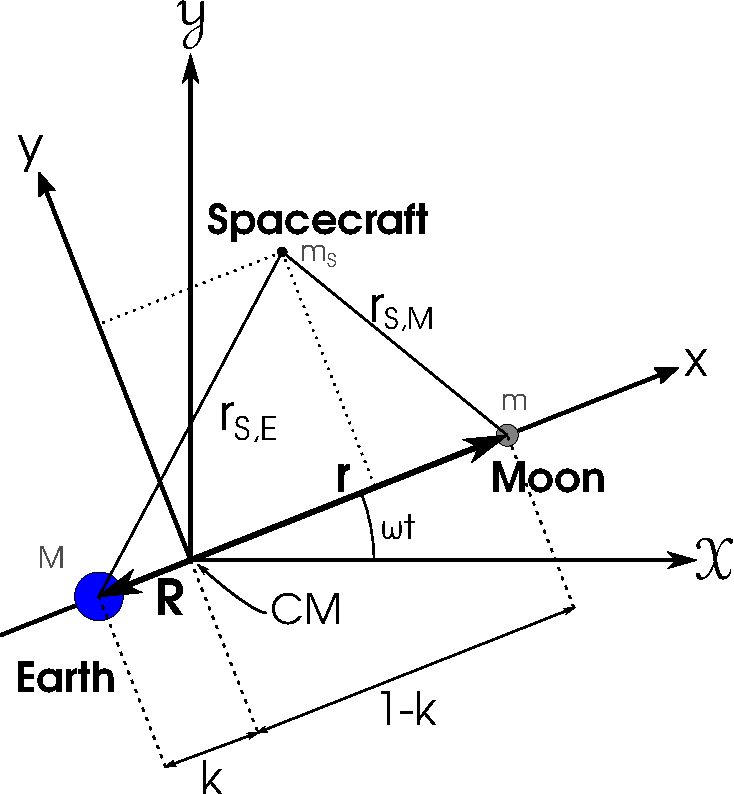
\includegraphics[scale=0.75]{fig/r3b.pdf}
\caption{Restricted three-body problem. Two coordinate systems both with center of mass as origin: $(\mathscr{X},\mathscr{Y})$ is a stationary interial frame, $(x,y)$ is a co-rotating non-interial frame that rotates with the moon at angular frequency $\omega$. $M =$ mass of Earth, $m =$ mass of Moon, $\vec{R} =$ vector from CM to earth, $\vec{r} =$ vector from CM to Moon, $m_s =$ mass of spacecraft, $r_{S,E} =$ distance from spacecraft to Earth, $r_{S,M} =$ distance from spacecraft to Moon. In the dimensionless variables we introduce later, unit distance is $R+r$, which makes the dimensionsless constant $k = \text{the CM-Earth distance} = \dfrac{R}{R+r} = $ and $1-k = \text{the CM-Moon distance} = \dfrac{r}{R+r}$}
\label{fig:r3b}
\end{figure}
We define two cartesian coordinate systems, both with their origin in the Moon-Earth center of mass (CM). The $(\mathscr{X},\mathscr{Y})$ system is a stationary inertial frame, and the $(x,y)$ system is co-rotating with the Earth and the Moon in their orbits, see Figure \ref{fig:r3b}.

We have two choices of coordinate systems to use for the Lagrangian:
\begin{enumerate}
    \item If we choose the inertial frame of reference, $T$ is straight forward, but distances in the $V$ becomes bothersome, albeit we can use the straightforward gravitational potential function.
    \item If we choose the rotating $(x,y)$ system, distances for $V$ is straight forward but then we either have to use polar coordinates, use an effective potential function instead of the standard gravitational potential, or use cartesian coordinates but find a coordinate transformation $X(x,y)$ and $Y(x,y)$.
\end{enumerate}
I arbitrarily choose the latter option: use $(x,y)$ coordinates and find $X(x,y)$ and $Y(x,y)$ transformation.

The distances between spacecraft and Earth/Moon are delightfully easy to work out:
\begin{align}
r_{S,E} = \sqrt{(x+R)^2+y^2}, \\
r_{S,M} = \sqrt{(x-r)^2+y^2},
\end{align}
where R and r are the distances from CM to Earth and Moon, respectively (see \ref{fig:r3b}).

In anticipation for calculating the kinetic energy of the system, we need the quantity
\begin{align}
\dot{\mathscr{X}}^2 + \dot{\mathscr{Y}}^2.
\end{align}
In matrix notation the coordinate transform between $(\mathscr{X},\mathscr{Y})$ and $(x,y)$ is obtained by the multiplication of the rotation matrix on the inertial frame coordinates
\begin{align}
\nonumber &\begin{bmatrix}
  \mathscr{X} \\
  \mathscr{Y}
\end{bmatrix}
=
\begin{bmatrix}
  \cos{\omega t} & -\sin{\omega t} \\
  \sin{\omega t} & \cos{\omega t}
\end{bmatrix}
\begin{bmatrix}
  x \\
  y
\end{bmatrix} \\[0.2cm]
\label{eq:coordinate-transform}
\Rightarrow
\begin{split}
&\begin{cases}
\ \mathscr{X} = x\cos{\omega t} - y\sin{\omega t} \\
\ \mathscr{Y} = x\sin{\omega t} + y\cos{\omega t}
\end{cases}
\end{split}.
\end{align}
By using the pythagorean trigonometric identity\footnote{$\cos^2{\theta} + \sin^2{\theta} = 1$} a number of times (see appendix \ref{app:coordinate-transform} for detailed derivation) we obtain
\begin{align}
\mathscr{\dot{\mathscr{X}}}^2 + \mathscr{\dot{\mathscr{Y}}}^2 = (\dot{x}-\omega y)^2 + (\dot{y}+\omega x)^2.
\end{align}
Now we can really see another convenience of the $(x,y)$ coordinate system: it eliminates explicite time-dependence of $L$ that would have been there in $V$ in the $(\mathscr{X},\mathscr{Y})$ system.

We are now ready to derive the equations of motion using the procedure from chapter 3.4.
\subsection{Equations of Motion}
The kinetic energy is
\begin{align}
\label{eq:r3b-T}
\nonumber T &= \dfrac{1}{2} m_s (\dot{\mathscr{X}}^2 + \dot{\mathscr{Y}}^2) \\
&= \dfrac{1}{2} m_s \left[(\dot{x}-\omega y)^2 + (\dot{y}+\omega x)^2\right].
\end{align}
The potential energy is
\begin{align}
\nonumber V &= - G m_s \left(\dfrac{M}{r_{S,E}} + \dfrac{m}{r_{S,M}}\right) \\
&= - G m_s \left(\dfrac{M}{\sqrt{(x+R)^2+y^2}} + \dfrac{m}{\sqrt{(x-r)^2+y^2}}\right).
\end{align}
The Lagrangian is
\begin{align}
\begin{split}
L &= T - V \\
&= \dfrac{1}{2} m_s \left[(\dot{x}-\omega y)^2 + (\dot{y}+\omega x)^2\right] \\
&+ G m_s \left(\dfrac{M}{\sqrt{(x+R)^2+y^2}} + \dfrac{m}{\sqrt{(x-r)^2+y^2}}\right).
\end{split}
\end{align}
The generalized momenta are
\begin{align}
p_x = \dfrac{\partial L}{\partial \dot{x}} = m_s(\dot{x} - \omega y), \\
p_y = \dfrac{\partial L}{\partial \dot{y}} = m_s(\dot{y} + \omega x).
\end{align}
From which we get the $\dot{x}(x,p_x)$ and $\dot{y}(y,p_y)$
\begin{align}
\dot{x} = \dfrac{p_x}{m_s} + \omega y, \\
\dot{y} = \dfrac{p_y}{m_s} - \omega x \ .
\end{align}
The Hamiltonian is
\begin{align}
H &= \sum\limits_{i=1}^n p_i \dot{q_i} - L \\[0.6cm]
&= \dfrac{p_x^2 + p_y^2}{m_s} + p_x\omega y - p_y\omega x - \dfrac{1}{2} m_s \left[\left(\dfrac{p_x}{m_s}\right)^2 + \left(\dfrac{p_y}{m_s}\right)^2\right] \\
&- G m_s \left(\dfrac{M}{\sqrt{(x+R)^2+y^2}} + \dfrac{m}{\sqrt{(x-r)^2+y^2}}\right) \nonumber \\[0.6cm]
&= \dfrac{p_x^2 + p_y^2}{2 m_s} + p_x\omega y - p_y\omega x - G m_s \left(\dfrac{M}{\sqrt{(x+R)^2+y^2}} + \dfrac{m}{\sqrt{(x-r)^2+y^2}}\right).
\end{align}
so Hamilton's equations are
\begin{align}
\dot{x} &= +\dfrac{\partial H}{\partial p_x} = \dfrac{p_x}{m_s} + \omega y, \\[0.4cm]
\dot{y} &= +\dfrac{\partial H}{\partial p_y} = \dfrac{p_y}{m_s} - \omega x, \\[0.4cm]
\dot{p}_x &= -\dfrac{\partial H}{\partial x} = \omega p_y - G m_s \left[-\dfrac{M(x+R)}{((x+R)^2+y^2)^{3/2}} + \dfrac{m(x-r)}{((x-r)^2+y^2)^{3/2}} \right], \\[0.4cm]
\dot{p}_y &= -\dfrac{\partial H}{\partial y} = -\omega p_x - G m_s \left[- \dfrac{M y}{((x+R)^2+y^2)^{3/2}} - \dfrac{m y}{((x-r)^2+y^2)^{3/2}}\right].
%\end{split}
\end{align}
By appropriate choice of units we can render the equations dimensionless.

A characteristic distance can be the Earth-Moon distance so:
\begin{align}
\text{One unit distance} = R+r .
\end{align}
A natural choice for the characteristic time is the moon's orbital period. Because the time dimension is present in the equations as $\omega$ we use Kepler's third law to express: \cite{Murray1999}
\begin{align}
\text{One unit time} = \dfrac{1}{\omega} = \sqrt{\dfrac{(R+r)^3}{G(M+m)}}.
\end{align}
The momentums $p_x$, $p_y$ of the spacecraft are going to be proportional with the spacecraft's mass $m_s$, so let's choose:
\begin{align}
\text{One unit mass} = m_s.
\end{align}
With these we can calculate:
\begin{align}
\nonumber \text{One unit momentum} &= \text{One unit velocity} = (\text{unit mass})\dfrac{\text{unit distance}}{\text{unit time}} \\[0.3cm]
\nonumber &= m_s(R+r)\sqrt{\dfrac{G(M+m)}{(R+r)^3}} \\[0.3cm]
&= m_s \sqrt{\dfrac{G(M+m)}{(R+r)}}.
\end{align}
We can now non-dimensionalize all the equations and get (see appendix \ref{app:non-dimensionalization})
\begin{empheq}[box=\widefbox]{align}
\label{eq:H-x}
\dot{X} = P_x + Y
\end{empheq}

\begin{empheq}[box=\widefbox]{align}
\label{eq:H-y}
\dot{Y} = P_Y - X
\end{empheq}

\begin{empheq}[box=\widefbox]{align}
\label{eq:H-px}
\dot{P_x} = P_y - \dfrac{(1-k)(X+k)}{((X+k)^2+Y^2)^{3/2}} - \dfrac{k(X-1-k)}{((X-1-k)^2+Y^2)^{3/2}}
\end{empheq}

\begin{empheq}[box=\widefbox]{align}
\label{eq:H-py}
\dot{P_y} = -P_x - \dfrac{(1-k)Y}{((X+k)^2+Y^2)^{3/2}} - \dfrac{k Y}{((X-1-k)^2+Y^2)^{3/2}} ,
\end{empheq}
where $T$, $X$, $Y$, $P_x$ and $P_y$ are our dimensionless variables, see appendix \ref{app:non-dimensionalization} for details.

For the rest of the time we will denote the non-dimensionalized units simply as $x,y,p_x,p_y$ instead of $X,Y,P_x,P_y$ for readability.

To reiterate, we have chosen units such that
\begin{align}
\text{unit length} &= \SI{3.85e5}{\km}, \\
\text{unit time} &= \SI{4.3484}{\days}, \\
\text{unit velocity} &= \SI{1.025}{\km/\s}.
\end{align}
Since all of the conditions in subsection \ref{ch:HvsE} are fulfilled, we have that $H=E$ and since $H$ does not depend explicitely on time, the Hamiltonian, and thus the energy, is conserved.
